\section{1174067 - Kaka Kamaludin}
\subsection{Teori}
\subsubsection{Klasifikasi Teks}
\hfill\break
Klasifikasi teks merupakan sebuah model yang biasa digunakan untuk untuk mengkategorikan sebuah teks ke dalam kelompok-kelompok yang lebih terorganisir. Jadi untuk setiap kalimat yang di masukan ke dalam mesin, mesin tersebut akan menjadikan setiap kata dari kalimat tersebut menjadi sebuah kolom. Untuk ilustrasinya bisa dilihat pada gambar berikut : 

\begin{figure}[H]
\centering
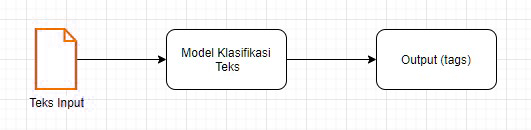
\includegraphics[width=4cm]{figures/1174067/4/1.jpg}
\caption{Klasifikasi Teks.}
\end{figure}

\subsubsection{Jelaskan mengapa hal ini bisa terjadi, klasifikasi bunga tidak bisa digunakan untuk machine learning}
\hfill\break
Karena machine learning tidak dapat menampilkan inputan sesuai dengan apa yang kita inputkan. Karena inputan tersebut serupa namun mesin memberikan output yang berbeda, biasanya output atau error ini disebut dengan istilah noise. Untuk contoh sederhananya misalkan kita inputkan salah satu label yang terdapat pada bunga, output yang dihasilkan oleh mesin tersebut ialah label yang lain. Itu dikarenakan bunga banyak jenis yang serupa namun tidak sama. Untuk ilustrasinya bisa dilihat pada gambar berikut: 

\begin{figure}[H]
\centering
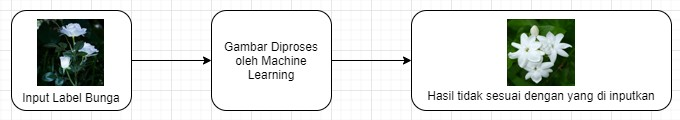
\includegraphics[width=4cm]{figures/1174067/4/2.jpg}
\caption{Klasifikasi Bunga.}
\end{figure}

\subsubsection{Jelaskan bagaimana yang dimaksud dengan teknik pembelajaran mesin pada teks yang digunakan}
\hfill\break
Teknik yang digunakan pada youtube salah satunya ialah keywords. Dengan keywords tersebut mesin dapat memberikan video sesuai dengan keyword yang kita inputkan pada kolom pencarian. Teknik pembelajarannya tergantung user memberikan input teks seperti apa, karena pada youtube itu sendiri akan menyesuaikan dengan apa yang biasa kita inputkan dan akan memfilter video secara otomatis sesuai dengan keyword yang biasa kita inputkan. Contoh ilustrasi sederhananya seperti berikut:

\begin{figure}[H]
\centering

\includegraphics[width=4cm]{figures/1174067/4/3.jpg}
\caption{Klasifikasi Teks pada Youtube.}
\end{figure}

\subsubsection{Vektorisasi Data}
\hfill\break
Vektorisasi data ialah suatu pemecahan atau pembagian data berupa teks, sebagai contoh terdapat 5 paragraf, data teks tersebut di pecah menjadi kalimat-kalimat yang lebih sederhana, lalu di pecah lagi menjadi kata untuk setiap kalimatnya. 

\subsubsection{Bag of Words}
\hfill\break
Representasi penyederhanaan sebuah kalimat atau perhitungan setiap kata pada suatu kalimat dengan presentase berapa kali muncul kata tersebut untuk setiap kalimatnya. Contoh ilustrasi sederhananya seperti berikut: 

\begin{figure}[H]
\centering
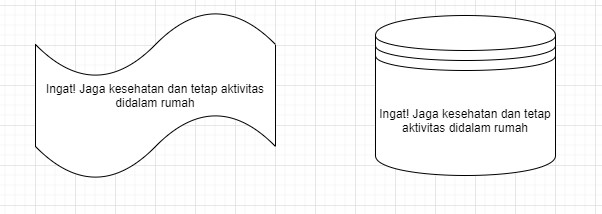
\includegraphics[width=4cm]{figures/1174067/4/4.jpg}
\caption{Bag of Words.}
\end{figure}

\subsubsection{TF-IDF}
\hfill\break
TF-IDF merupakan metode untuk menghitung bobot setiap kata pada suatu kalimat yang paling sering digunakan. TF-IDF ini akan menghitung nilai Term Frequency dan Inverse Document Frequency pada setiap kata dalam setiap kalimat yang muncul dengan diimbangi dengan jumlah dokumen dalam korpus yang mengandung kata. Contoh ilustrasi sederhananya seperti gambar berikut: 

\begin{figure}[H]
\centering
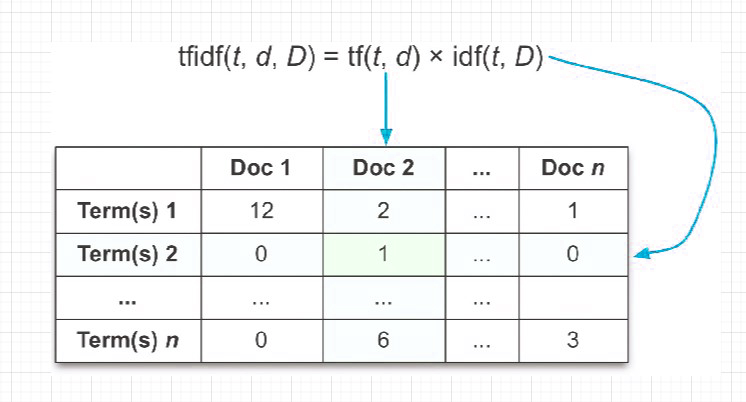
\includegraphics[width=4cm]{figures/1174067/4/5.jpg}
\caption{TF-IDF.}
\end{figure}

\subsection{Praktek}
\subsubsection{buat aplikasi klasifikasi sederhana menggunakan pandas, buat data dummy format csv sebanyak 500 baris dan melakukan load ke dataframe panda.jelaskan arti setiap baris kode yang dibuat(harus beda dengan teman sekelas)}
\hfill\\
\lstinputlisting[firstline=8, lastline=9, caption={kodingan praktek no. 1},captionpos=b]{src/1174067/4/1174067.py}
	\begin{figure}[H]
	\centering
		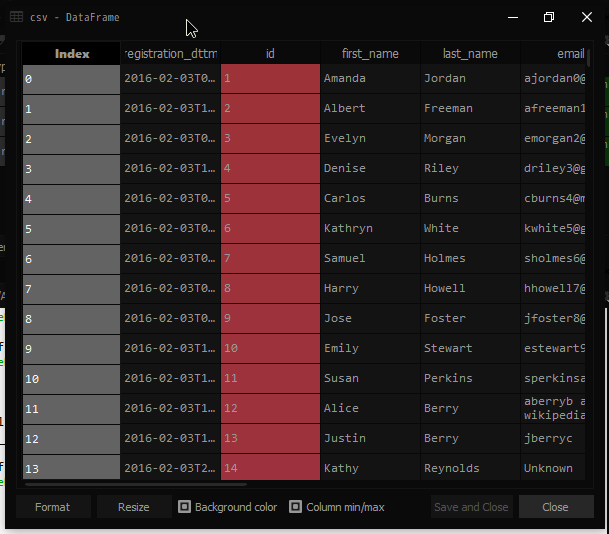
\includegraphics[width=8 cm]{figures/1174067/4/7.png}
	\caption{hasil praktek soal no. 1}
	\end{figure}


\subsubsection{dari dataframe tersebut dipecah menjadi dua dataframe yaitu 450 row pertama dan 50 row sisanya(harus beda dengan teman sekelas)}
\hfill\\
\lstinputlisting[firstline=11, lastline=11, caption={kodingan praktek no. 2},captionpos=b]{src/1174067/4/1174067.py}
	\begin{figure}[H]
	\centering
		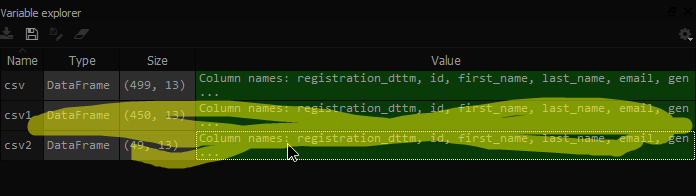
\includegraphics[width=8 cm]{figures/1174067/4/8.png}
	\caption{hasil praktek soal no. 2}
	\end{figure}

\subsubsection{praktekkan vektorisasi dan klasifikasi dari data(NPM mod 4, jika 0 maka ketty perry, 1 LMFAO, 2 Eminem, 3 Shakira) dengan Decission Tree. Tunjukkan keluaranya dari komputer sendiri dan artikan maksud luaran yang di dapatkan}
\hfill\\
\lstinputlisting[firstline=9, lastline=9, caption={1174067 mod 4},captionpos=b]{src/1174067/4/1174067-2.py}

\lstinputlisting[firstline=12, lastline=36, caption={kodingan praktek no. 3},captionpos=b]{src/1174067/4/1174067-2.py}
	\begin{figure}[H]
	\centering
		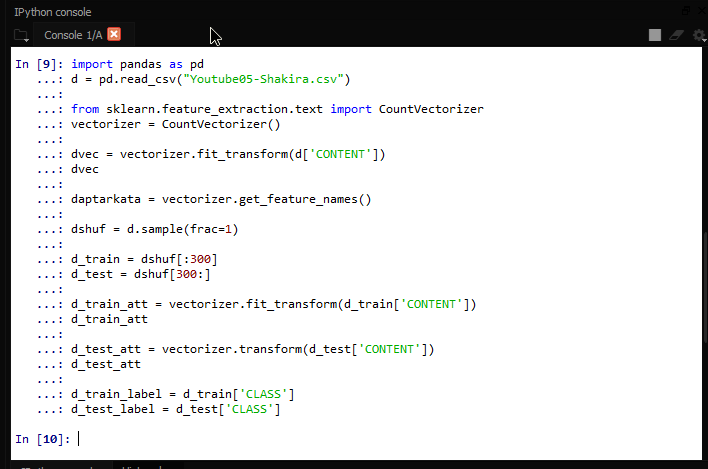
\includegraphics[width=8 cm]{figures/1174067/4/9.png}
	\caption{hasil praktek soal no. 3(1)}
	\end{figure}
	Vektorisasi data content dari file Youtube04\_Shakira.CSV
	\begin{figure}[H]
	\centering
		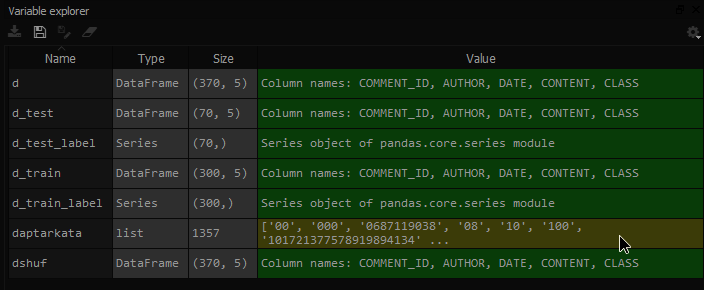
\includegraphics[width=8 cm]{figures/1174067/4/10.png}
	\caption{hasil praktek soal no. 3(2)}
	\end{figure}
	
\subsubsection{Cobalah klarifikasikan dari data vektorisasi yang di tentukan di nomor sebelumnya dengan klasifikasi SVM. Tunjukkan keluaranya dari komputer sendiri dan artikan maksud setiap luaran yang didapatkan}
\hfill\\
\lstinputlisting[firstline=47, lastline=50, caption={kodingan praktek no. 4},captionpos=b]{src/1174067/4/1174067-2.py}
	\begin{figure}[H]
	\centering
		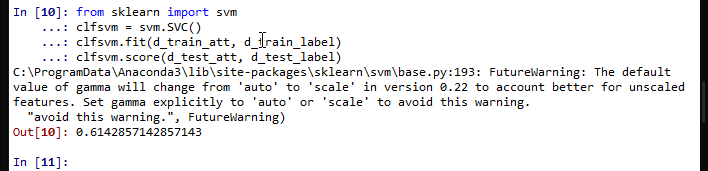
\includegraphics[width=8 cm]{figures/1174067/4/11.png}
	\caption{hasil praktek soal no. 4}
	\end{figure}

\subsubsection{Cobalah klasifikasikan dari data vektorisasi yang ditentukan dari nomor sebelumnya dengan klasifikasi Decision Tree. Tunjukan keluaranya dari komputer sendiri dan artikan maksud setiap luaran yang didapatkan}
\hfill\\
\lstinputlisting[firstline=40, lastline=43, caption={kodingan praktek no. 5},captionpos=b]{src/1174067/4/1174067-2.py}
	\begin{figure}[H]
	\centering
		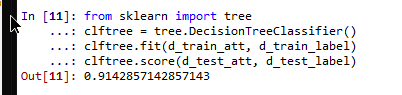
\includegraphics[width=8 cm]{figures/1174067/4/12.png}
	\caption{hasil praktek soal no. 5}
	\end{figure}

\subsubsection{Plotlah confusion matrix dari praktek modul ini menggunakan matplotlib.Tunjukkan keluarannya dari komputer sendiri dan artikan maksud setiap luaran yang didapatkan.}
\hfill\\
\lstinputlisting[firstline=61, lastline=106, caption={kodingan praktek no. 6(1)},captionpos=b]{src/1174067/4/1174067-2.py}
	\begin{figure}[H]
	\centering
		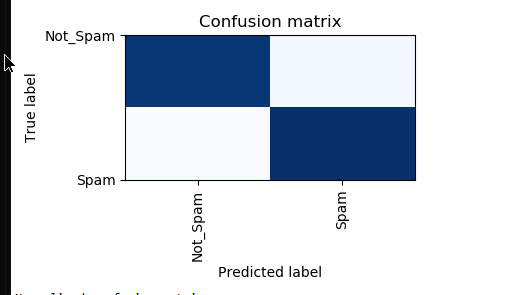
\includegraphics[width=8 cm]{figures/1174067/4/13.png}
	\caption{hasil praktek soal no. 6(1)}
	\end{figure}
	Plot confusion matrix dari klasifikasi Decission Tree.
\lstinputlisting[firstline=110, lastline=159, caption={kodingan praktek no. 6(2)},captionpos=b]{src/1174067/4/1174067-2.py}
	\begin{figure}[H]
	\centering
		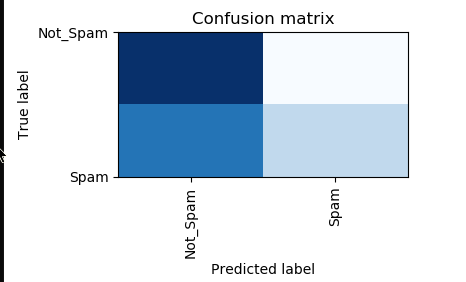
\includegraphics[width=8 cm]{figures/1174067/4/14.png}
	\caption{hasil praktek soal no. 6(2)}
	\end{figure}
	Plot confusion matrix dari klasifikasi SVM.
\lstinputlisting[firstline=163, lastline=211, caption={kodingan praktek no. 6(3)},captionpos=b]{src/1174067/4/1174067-2.py}
	\begin{figure}[H]
	\centering
		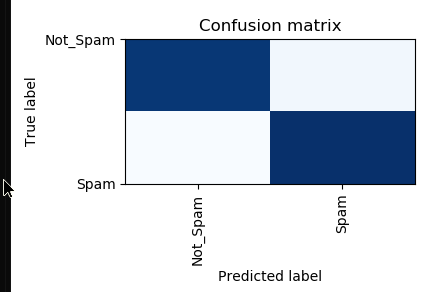
\includegraphics[width=8 cm]{figures/1174067/4/15.png}
	\caption{hasil praktek soal no. 6(3)}
	\end{figure}
	Plot confusion matrix dari klasifikasi Random Forest.
	
\subsubsection{jalankan program cross validaiton pada bagian teori bab ini. Tunjukkan keluarannya dari komputer sendiri dan artikan maksud setiap luaran yang didapatkan.}
\hfill\\
\lstinputlisting[firstline=215, lastline=224, caption={kodingan praktek no. 7},captionpos=b]{src/1174067/4/1174067-2.py}
	\begin{figure}[H]
	\centering
		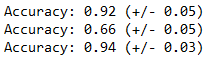
\includegraphics[width=5 cm]{figures/1174067/4/16.png}
	\caption{hasil praktek soal no. 7}
	\end{figure}

\subsubsection{Buatlah program pengamatan komponen informasi pada bagian teori bab ini. Tunjukkan keluarannya dari komputer sendiri dan artikan maksud setiap luaran yang didapatkan.}
\hfill\\
\lstinputlisting[firstline=228, lastline=241, caption={kodingan praktek no. 8},captionpos=b]{src/1174067/4/1174067-2.py}
	\begin{figure}[H]
	\centering
		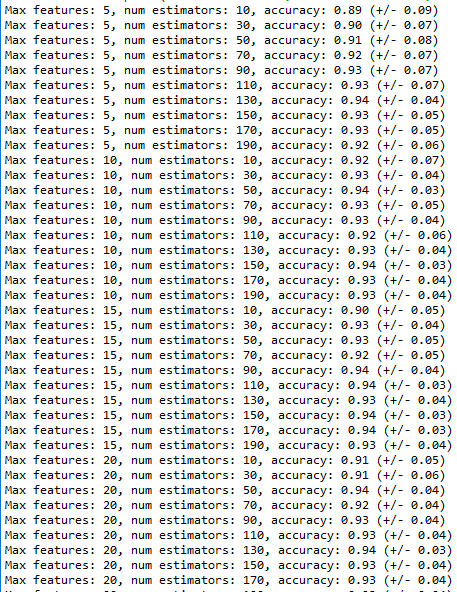
\includegraphics[width=8 cm]{figures/1174067/4/17.png}
	\caption{hasil praktek soal no. 8(1)}
	\end{figure}
	\hfill\\
	\begin{figure}[H]
	\centering
		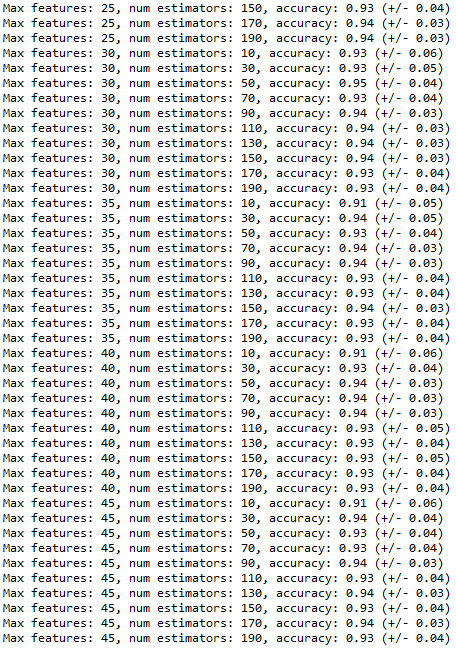
\includegraphics[width=8 cm]{figures/1174067/4/18.png}
	\caption{hasil praktek soal no. 8(2)}
	\end{figure}
	
\subsection{Penanganan Error}
\begin{enumerate}
	\item FileNotFoundError
	\begin{figure}[H]
		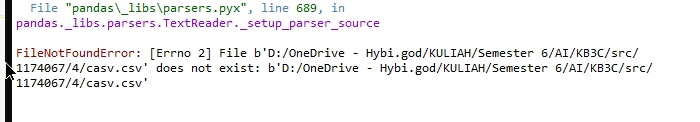
\includegraphics[width=4cm]{figures/1174067/4/error1.jpg}
		\centering
		\caption{FileNotFoundError}
	\end{figure}
	\item Cara Penangan Error
	\begin{itemize}
		\item FileNotFoundError
		\hfill\break
		Dengan menyesuaikan letak file csv pada codingannya, sehingga dapat  di baca atau dipanggil file csvnya.
	\end{itemize}
\end{enumerate}

\subsection{Link Youtube}
https://www.youtube.com/playlist?list=PL4dhp4u89PHbhX9jrGyM3N12gmwhY3uIe